\section{Graph Convolutional Networks}

The recent popularity of convolutional neural networks (\cite{40k}), and their
success in classifying images and in other tasks with a striking accuracy, has intrigued the scientific
community with the question of whether -at least a variant of them- can be leveraged in learning tasks
of graph networked data. The use of graph structures in computer
vision (\cite{survey}), as well as in the representation of social networks
(\cite{kleinberg_book}), has made this task look appealing and worth of investigation.
However, using convolutional neural networks for
networked data directly is not a straightforward task and it poses significant
challenges.\\

\spara{Challenges in Graph Convolutional Networks} First and foremost,
as CNNs were mainly used for image classification, they assume that
data lie on a regular grid in a geometric space (most commonly
Euclidean). On the contrary, graph data are a typical form of unordered data that lie in
an irregular domain. Also, the heavy-tailed distribution of node degrees
in real networks \cite{smth} makes the filtering-convolution part difficult,
as it is not easy to define a constant-sized neighborhood and apply a
localized filter, as in the traditional CNN case. Similarly, one needs to find an analogue of the pooling stage.\\

\spara{Convolution in graphs} First efforts to address the above mentioned issues
by Bruna et al. \cite{Lecun} and introduce the architecture of CNNs to networked data,
mainly draw from the field of Graph Signal Processing \cite{shuman}.
Graphs are generally considered undirected and their representation is given
through their \textbf{Laplacian $L = D -A$} or more commonly the normalized
\textbf{Laplacian $L = I_n - D^{-\frac{1}{2}}AD^{-\frac{1}{2}}$}. As this matrix
is real, symmetric and positive semidefinite, it admits an eigenvector
decomposition $L=U\Lambda U^T$, where $U$ is a square orthonormal matrix with
the eigenvectors as its columns, and $\Lambda$ is the diagonal matrix of eigenvalues.
Letting $x\in \mathbb{R}^{n}$ be a feature vector of the nodes of a graph,
the {\em Graph Fourier Transform} is then defined as $\hat{x}=U^T x \in \mathbb{R}^n$
and its inverse as $x = U\hat{x}$. The \textbf{convolution operator} on a graph
$\mathcal{G}$ is defined on the Fourier domain, as:
\begin{equation*}
x *_{\mathcal{G}} y = U((U^T x)\odot (U^T y))
\end{equation*}
where $\odot$ denotes the element-wise Hadamard product.\\
Therefore, a signal $x$ is filtered by $g_{\theta}$, as:\\
\begin{equation}
y = g_{\theta}(L)x = g_{\theta} (U\Lambda U^T)x = U g_{\theta}(\Lambda ) U^T x
\end{equation}
where $g_{\theta}(\Lambda) = diag(\theta)$ is a non-parametric filter.\\
This approach has, however, the following limitations:
\begin{itemize}
\item [1.] Filters are not localized
\item [2.] Their learning complexity scales with the dimensionality of the data $O(n)$
\item [3.] The computational cost of filtering is high ($O(n^2)$), due to the
multiplication with the Fourier basis $U$.
\end{itemize}

\subsubsection*{Spectral CNN using Chebyshev Polynomials}
Deferrard et al. \cite{defferard} were the first to propose a way to deal with
the above issues.\\

\spara{Localized Filter} First of all, they propose the use of a polynomial filter:\\
\begin{equation}
g_{\theta}(\Lambda ) = \sum_{k=0}^{K-1}\theta_k \Lambda^k
\end{equation}
where the parameter $\theta \in \mathbb{R}^K$ is a vector of polynomial
coefficients. As $(L^K)_{i,j} = 0$ whenever $d_{\mathcal{G}}(i,j)>K$, these
spectral filters are $K$-localized.\\

\spara{Learning complexity} Their learning complexity is equal to the support
size of the filter, i.e. $O(K)$, as in conventional CNNs.\\

\spara{Computational cost of filtering} As mentioned earlier, due to the
multiplication of the filter with the Fourier basis $U$, the computational cost
is relatively high, $O(n^2)$. For this reason, they express the filter as a
Chebyshev polynomial of order $k$, that can be computed using the recurrence
$T_k(x) = 2xT_{k-1}(x)-T_{k-2}(x)$ with $T_o = 1$ and $T_1 = x$. Thus, the whole
filtering operation can be written as $y = g_{\theta}(L)x =
\sum_{k=0}^{K-1}\theta_k T_k (\widetilde{\Lambda })x$, where $T_k (\Lambda ) \in
\mathbb{R}^{nxn}$ is the Chebyshev polynomial of order $k$ evaluated at the
scaled Laplacian $\widetilde{\Lambda} = 2L/\lambda_{max} - I_n$, using the
recurrence $\bar{x}_k = 2\widetilde{\Lambda}\bar{x}_{k-1} - \bar{x}_{k-2}$, with
$\bar{x}_0 = x$ and $\bar{x}_1 = \widetilde{\Lambda}x$. The cost of the
filtering operation becomes then $O(K|E|)$, as it is a multiplication of a
sparse matrix with a column vector of size $K$.\\

\spara{Graph Coarsening and Pooling}
Pooling on traditional convolutional neural networks, is performed usually on a
patch of neighboring pixels on an image. However, in graphs, we can not explicitly
define this notion of neighborhood as in a Euclidean grid. Therefore, the authors of
this paper propose a multilevel clustering approach, that not only clusters
similar vertices - in a topological fashion- together, but also produces coarser
versions of the graph at each level, closely mimicking the pooling operation of traditional
CNNs. The multilevel clustering algorithm chosen is Graclus \cite{Kulis}.\\
In order to perform pooling in a fast and memory efficient manner, nodes are
organized in a balanced binary tree. Specifically, after coarsening, each node
has either two childer, if it was matched at the finer level, or one, if it was
not. Those singleton nodes are paired with fake nodes, having a neutral value
- with respect to the activation function - as their input. A visualization of this
operation, can be seen in Fig.~\ref{pooldef}.
\begin{figure}
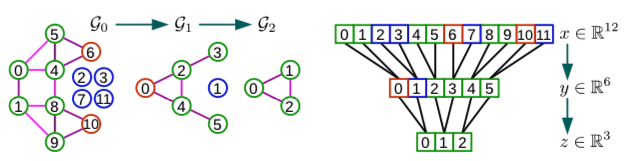
\includegraphics[scale=0.5]{pooling_def}
\caption{Pooling operation, using Greclus clustering and arranging nodes in a
balanced binary tree. Blue nodes are added fake nodes}
\label{pooldef}
\end{figure}
\subsubsection*{$1^{st}$ order approximation and semi-supervised classification}
Kipf and Welling \cite{kipf} build upon the previous work of Defferrard
presented above, introducing simplifications that allow for significantly faster training
times and higher predictive accuracy. Also, in their framework, they introduce a
way to perform semi-supervised classification tasks, so that their model has the
ability to classify nodes, even if most samples of the dataset are unlabeled.\\
A very simple form of a later -wise propagation rule would be of the form:
\begin{equation*}
f(H^{(l+1)},A) = \sigma(AH^{(l)}W^{(l)})
\end{equation*}
where $W^{(l)}$ is the weight matrix of the $l$-layer of the neural network,
$H^{(l)}$ is the matrix of activations at the previous layer, and $\sigma(\cdot
)$ could be  a non-linear activation function, like ReLU.\\
However, this propagation rule, has some limitations. First of all, a node only
sums features of neighboring nodes, but not itself. In order to solve this issue, we augment
the adjacency matrix with self-loops, giving $\widetilde{A} = A + I_N$. Secondly, as
long as $A$ is not normalized, this summation will change the scale of features,
hence we need a symmetric normalization, i.e.
$D^{-\frac{1}{2}}AD^{-\frac{1}{2}}$ to get rid of this problem. Thus, the
propagation rule now becomes:\\
\begin{equation}
H^{(l+1)} =
\sigma(\widetilde{D}^{-\frac{1}{2}}\widetilde{A}\widetilde{D}^{-\frac{1}{2}}H^{(l)}W^{(l)})
\end{equation}
As most real-world networks (e.g. social networks, citation networks, knowledge
graphs) have distributions close to power-law, the authors restrict
the Chebyshev filters proposed by (\cite{mddef}) to $K=1$, expecting that this
simplification will allow them to build deeper models and avoid any possible
overfitting on local neighborhood structures. Setting, further, $\theta_0 =
-\theta_1 = \theta$, leaves their model with only a single parameter to learn.
Thus, the convolution operation is now:

\[
g_\theta * x \approx \theta (\widetilde{D}^{-\frac{1}{2}}\widetilde{A}\widetilde{D}^{-\frac{1}{2}})
x
\]
For a signal $X \in \mathbb{R}^{NxC}$, $F$ filters or feature maps, the
complexity of the above operation is now $O(|E|FC)$.\\

\spara{Semi-supervised classification}
By conditioning the model $f(X,A)$ on both the data $X$ and the adjacency
matrix $A$, this model can be used on semi-supervised tasks, where not all
samples are labeled, expecting that the adjacency matrix will contain enough
information not present in the data matrix $X$.\\
Thus, for semi-supervised classification a \textbf{cross-entropy loss} over all labeled
examples is used:
\begin{equation}
\mathcal{L} = - \sum_{l\in \mathcal{Y_L}} \sum_{f=1}^{F} Y_{lf}lnZ_{lf}
\end{equation}
where $\mathcal{Y}_L$ is the set of labeled nodes.\\
Though this work seems to work well in practice, providing good results for
certain classification tasks in real networks (like citation networks), it has
some \textbf{limitations}:
\begin{enumerate}
\item It uses gradient descent for training, which is suitable only for dataset sizes that can fit in memory.
\item The single-parameter model and the absence of pooling operations make this work not suitable for IVC
tasks, like image segmentation, as in regular graphs. This results in sharing
the same kernel (up to a multiplication factor) across all layers and all units
in entire network (\cite{blogpost}) .
\item The recursive expansion of neighborhoods across layers incurs expensive computations, as for power-law graphs, a single
vertex can quickly fill up a large portion of the graph (\cite{fastgcn}).
\end{enumerate}

\subsubsection*{GraphSAGE}
GraphSAGE \cite{inductive} is a technique to embed nodes of large graphs into a
low-dimensional space, by using a neural network approach.\\
The key difference between GraphSAGE and the other approaches that we 've seen
so far, is that instead of learning a representation for every node, GraphSAGE
learns a function that generates embeddings by sampling and aggregating features
from node's local neighborhood.\\
\spara{The embedding algorithm} Algorithm 1~\ref{algo} describes the way
embeddings are generated. We present the algorithm under the assumption that
we have learned the parameters of the $K$ aggregator functions, as well as a
set of weight matrices $W^k$, which are used to propagate features between
different layers (search depths) of the model. We will describe later how these
parameters can be learned.
\begin{figure}[h!tb]
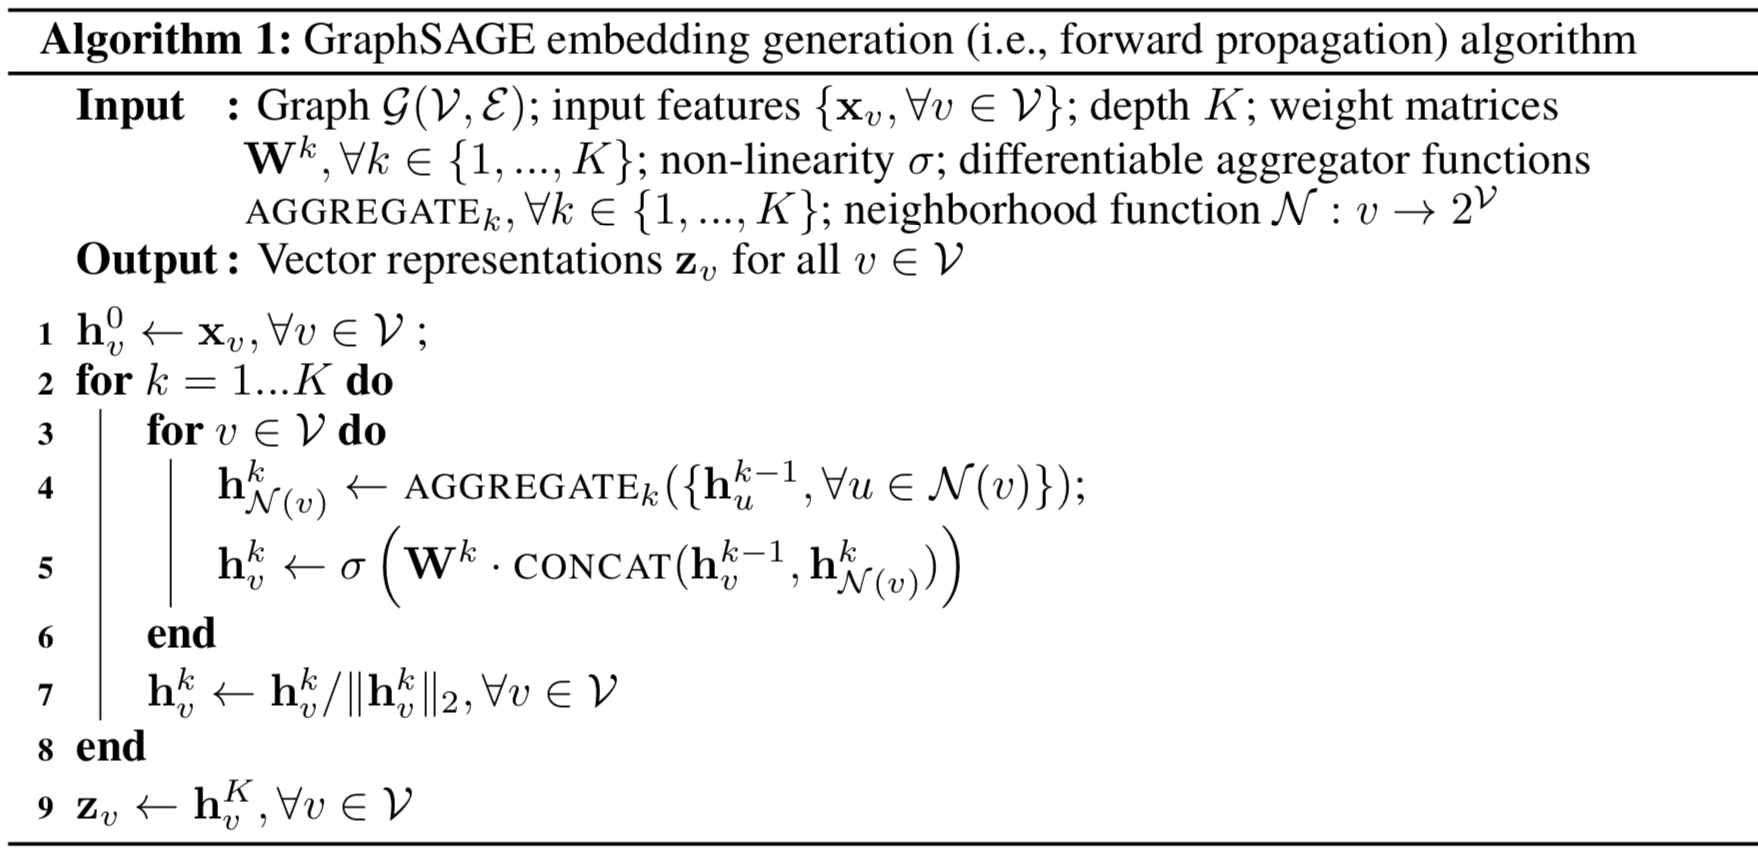
\includegraphics[scale=0.4]{sageEmbedding}
\label{algo}
\end{figure}
As we see on each iteration $K$, a node aggregates representations of the nodes
in its immediate neighborhood into a single vector. Then it concatenates this
vector with its current representation. This new vector is transformed using the weight matrix
$W^k$ and a non-linear activation function, before being used at the next step
of the algorithm. In order to keep the computational cost small, the authors
sample uniformly a fixed-size set of neighbors at each step.\\
\spara{Learning the parameters} While a different computational graph is
constructed for every node, the parameters $W^k$, as well the parameters of the
aggregator functions are shared across those different networks. Hence, we can
learn those parameters using stochastic gradient descend and back-propagation.
For an unsupervised setting, we can define a graph-loss function to the output
representations, while for completely supervised settings we can use different
loss functions, like the cross-entropy.
\spara{ Aggregator functions} The authors of this paper also propose a set of
aggregator functions that can be used by this model. Among them is $mean$, which
simply takes the average of the representations of neighboring nodes, and
$pooling$, where each neighbor's vector is independently fed through a
fully-connected neural network. Following this transformation, an elementwise
max-pooling operation is applied to aggregate information across the neighbor
set.

